%%%%%%%%%%%%%%%%%%%%%%%%%%%%%%%%%%%%%%%%%
% Beamer Presentation
% LaTeX Template
% Version 1.0 (10/11/12)
%
% This template has been downloaded from:
% http://www.LaTeXTemplates.com
%
% License:
% CC BY-NC-SA 3.0 (http://creativecommons.org/licenses/by-nc-sa/3.0/)
%
%%%%%%%%%%%%%%%%%%%%%%%%%%%%%%%%%%%%%%%%%

%----------------------------------------------------------------------------------------
%	PACKAGES AND THEMES
%----------------------------------------------------------------------------------------

\documentclass[xcolor=svgnames]{beamer}

\mode<presentation> {

% The Beamer class comes with a number of default slide themes
% which change the colors and layouts of slides. Below this is a list
% of all the themes, uncomment each in turn to see what they look like.

% \usetheme{default}
% \usetheme{AnnArbor}
% \usetheme{Antibes}
%\usetheme{Bergen}
% \usetheme{Berkeley}
% \usetheme{Berlin}
\usetheme{Boadilla}
% \usetheme{CambridgeUS}
% \usetheme{Copenhagen}
% \usetheme{Darmstadt}
% \usetheme{Dresden}
% \usetheme{Frankfurt}
% \usetheme{Goettingen}
% \usetheme{Hannover}
% \usetheme{Ilmenau}
% \usetheme{JuanLesPins}
% \usetheme{Luebeck}
% \usetheme{Madrid}
% \usetheme{Malmoe}
% \usetheme{Marburg}
% \usetheme{Montpellier}
% \usetheme{PaloAlto}
% \usetheme{Pittsburgh}
% \usetheme{Rochester}
% \usetheme{Singapore}
% \usetheme{Szeged}
% \usetheme{Warsaw}

% As well as themes, the Beamer class has a number of color themes
% for any slide theme. Uncomment each of these in turn to see how it
% changes the colors of your current slide theme.

% \usecolortheme{albatross}
% \usecolortheme{beaver}
%\usecolortheme{beetle}
% \usecolortheme{crane}
%  \usecolortheme{dolphin}
% \usecolortheme{dove}
% \usecolortheme{fly}
% \usecolortheme{lily}
% \usecolortheme{orchid}
% \usecolortheme{rose}
% \usecolortheme{seagull}
% \usecolortheme{seahorse}
% \usecolortheme{whale}
% \usecolortheme{wolverine}

% \setbeamertemplate{footline} % To remove the footer line in all slides uncomment this line
%\setbeamertemplate{footline}[page number] % To replace the footer line in all slides with a simple slide count uncomment this line

% \setbeamertemplate{navigation symbols}{} % To remove the navigation symbols from the bottom of all slides uncomment this line
}

\usepackage{graphicx} % Allows including images
\usepackage{booktabs} % Allows the use of \toprule, \midrule and \bottomrule in tables
\usepackage{tikz}
\usepackage{multicol}
\usepackage{wrapfig}
\usepackage{amsmath,amsthm,amssymb}
\usepackage{mathtools}
\DeclarePairedDelimiter\ceil{\lceil}{\rceil}
\DeclarePairedDelimiter\floor{\lfloor}{\rfloor}


\addtobeamertemplate{frametitle}{}{%
\begin{tikzpicture}[remember picture,overlay]
\node[anchor=north east,yshift=2pt] at (current page.north east) {
\includegraphics[height=0.8cm]{iiit-new.png}};
\end{tikzpicture}}

\setbeamercolor{title in head/foot}{bg=OrangeRed, fg=White}
\setbeamercolor{author in head/foot}{bg=RoyalBlue, fg=White}
\setbeamercolor{date in head/foot}{bg=SlateGray, fg=Black}

%----------------------------------------------------------------------------------------
%	TITLE PAGE
%----------------------------------------------------------------------------------------

\title[Discrete Structures]{Discrete Structures} % The short title appears at the bottom of every slide, the full title is only on the title page
\author{IIIT Hyderabad} % Your name
\institute[] % Your institution as it will appear on the bottom of every slide, may be shorthand to save space
{
Monsoon 2020 \\ % Your institution for the title page
\medskip
\textit{Tutorial 3} % Your email address
}
\date{September 23, 2020} % Date, can be changed to a custom date

\begin{document}

\begin{frame}
\titlepage % Print the title page as the first slide
\end{frame}

\begin{frame}
\frametitle{Introduction} % Table of contents slide, comment this block out to remove it
\tableofcontents % Throughout your presentation, if you choose to use \section{} and \subsection{} commands, these will automatically be printed on this slide as an overview of your presentation
\end{frame}

%----------------------------------------------------------------------------------------
%	PRESENTATION SLIDES
%----------------------------------------------------------------------------------------


%------------------------------------------------
\section{Questions}
%------------------------------------------------

%------------------------------------------------
\subsection{Question 0}
%------------------------------------------------
\begin{frame}
\frametitle{Question 0}
\textbf{0.2} Find the number of primes between 40 - 100 using PRT.
\\ \textbf{\underline{Sol:}} 
\begin{center}
    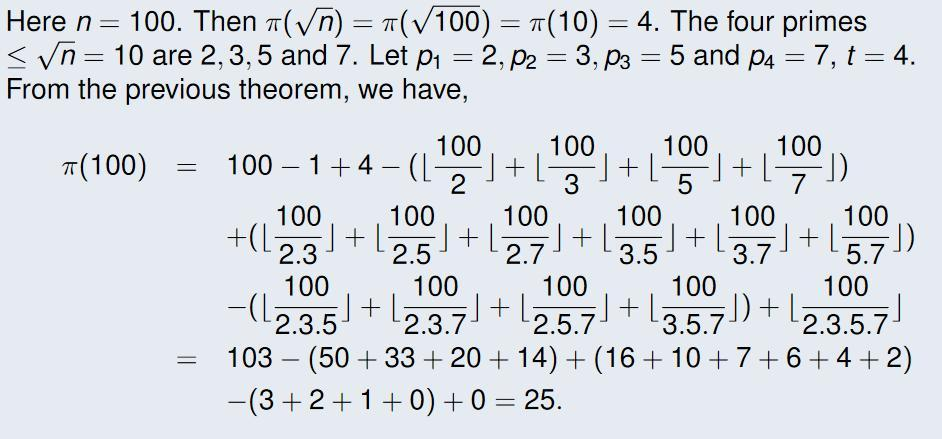
\includegraphics[width=0.8\linewidth]{photo_2020-09-23_00-54-28.jpg}
\end{center}
We have $\pi(6) = 3$, thus $\pi(40) = 40 - 1 + 3 - \floor{\frac{40}{2}} - \floor{\frac{40}{5}} - \floor{\frac{40}{3}} + \floor{\frac{40}{10}} + \floor{\frac{40}{6}} + \floor{\frac{40}{15}} - \floor{\frac{40}{30}}$ 
\\ $= 12$
\\ Thus we get number of primes is $25 - 12 = 13$.

\end{frame}



%------------------------------------------------
\subsection{Question 1}
%------------------------------------------------
\begin{frame}
\frametitle{Question 1}

Simplify the following - 
\begin{enumerate}
    \item $\big(A - (B \cup C)\big) \cap \big((B \cap C) - A\big)$
    \\ \textbf{\underline{Sol:}} 
    \begin{align*}
        & \big(A - (B \cup C)\big) \cap \big((B \cap C) - A\big)
        \\ &= \big(A \cap (B' \cap C')\big) \cap \big((B \cap C) \cap A'\big) & \ldots \ldots \{\text{ De Morgan's Laws }\}
    \end{align*}
    The above can be re arranged  using associative and commutative law as $ \big((A \cap A') \cap (B \cap B') \cap (C \cap C')\big)=  \phi \cap \phi \cap \phi = \phi$
    \item $(A \cap B') \cup (A' \cap B) \cup (A' \cap B')$
    \begin{align*}
        & (A \cap B') \cup (A' \cap B) \cup (A' \cap B')
        \\ & (A \cap B') \cup (A' \cap (B \cup B') & \ldots \ldots \{\text{ Associative Law }\}
        \\ & (A \cap B') \cup (A' \cap (U)) & \ldots \ldots \{\text{ A' $\cup$ A = U}\}
        \\ & (A \cap B') \cup (A') & \ldots \ldots \{\text{ A $\cap$ U = A }\}    
        \\ & (A \cup A') \cap (B' \cup  A') & \ldots \ldots \{\text{ Since commutative }\}        
        \\ & U \cup (B' \cap  A') = (B' \cap A') & \ldots \ldots \{\text{ A $\cup$ A' = U, U $\cup$ A = A }\}
    \end{align*}    
\end{enumerate}
\end{frame}
\subsection{Question 2}
\begin{frame}
\frametitle{Question 2}
\begin{multicols}{2}
\footnotesize{ 
\textbf{2.1} $A$ is the set of people who go to resort area for vacation, $B$ is the set of people who take cruise for vacation, $C$ is the set of people who go to national park for vacation. Suppose $|A| = 150, |B| = 100$ and $|C|=300$
}
\begin{figure}
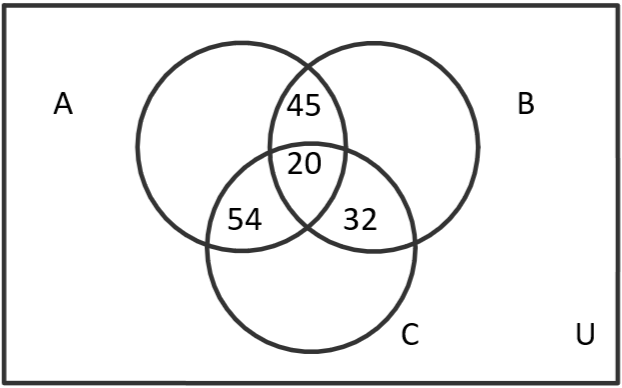
\includegraphics[width=0.5\linewidth]{dstut3q2.png}
\end{figure}
\footnotesize{
\textbf{a.} How many people only go to a resort area for vacation? \\\
\textbf{\underline{Sol:}} $|A| - |A \cap B|  - |A \cap C| + |A \cap B \cap C| = 31$
\textbf{b.} How many people only take a cruise for vacation? \\
\textbf{\underline{Sol:}} $|B| - |B \cap A|  - |B \cap C| + |A \cap B \cap C| = 3$
\textbf{c.} How many people only go to national park for vacation? \\
\textbf{\underline{Sol:}} $|C| - |C \cap A|  - |C \cap B| + |A \cap B \cap C| = 194$
\textbf{d.} How many people either go to a resort area or take a cruise for vacation but not national park? \\
\textbf{\underline{Sol:}} $|A| + |B| - |A \cap B| - |A \cap C| - |B \cap C| +  |A \cap B \cap C|  = 79$ \\
\textbf{e.} How many people use any of the 3 methods to take a vacation? \\
\textbf{\underline{Sol:}} $|A| + |B| + |C| - |A \cap B| - |A \cap C| - |B \cap C| +  |A \cap B \cap C|  = 379$
}
\end{multicols} 
\end{frame}

\begin{frame}
\frametitle{Question 2 (contd.)}
\begin{multicols}{2}
\small{
\textbf{2.2} Observe the values of the table and find the number of students who:
\begin{center}
\begin{figure}
    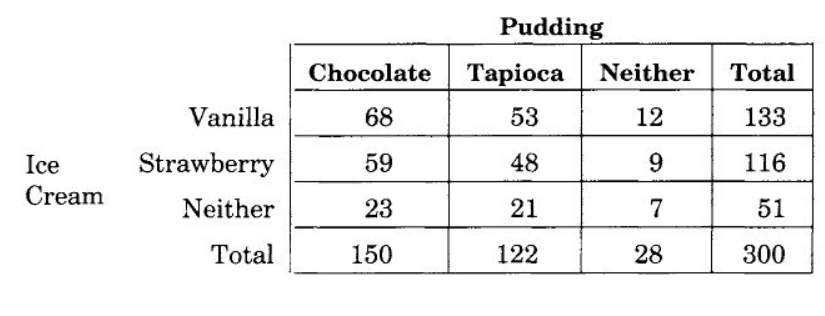
\includegraphics[width=\linewidth]{dstut3q2table.png}
\end{figure}
\end{center}
\textbf{a.} Like strawberry ice cream and tapioca pudding \\
\textbf{\underline{Sol:}} 48 \\
\textbf{b.} Do not like pudding \\
\textbf{\underline{Sol:}} 28 \\
\textbf{c.} Like at least one of the ice cream flavours \\
\textbf{\underline{Sol:}} $133 + 116 = 249$ \\
\textbf{d.} Like neither ice cream nor pudding\\
\textbf{\underline{Sol:}} 7 
\vspace{1mm}
\hline
\vspace{1mm}
\textbf{2.3} Mark the following as true or false:
\textbf{a.} $26 \in \mathbb{Z}  $ -- \textbf{True}\\
\textbf{b.} $-5 \in \mathbb{N}  $ -- \textbf{False} \\
\textbf{c.} $\sqrt{2} \notin \mathbb{Q} \cap \mathbb{R}$ -- \textbf{True} \\
\textbf{d.} $\mathbb{Z} \cup \mathbb{Q} = \mathbb{R}$ -- \textbf{False}\\
\textbf{e.} $\mathbb{R} \cap \mathbb{C} = \mathbb{R}$ -- \textbf{True}\\
}
\end{multicols}
\end{frame}

\begin{frame}
\frametitle{Quiz conducted on 22 Sept 2020}
Any doubts ?
\begin{enumerate}\setcounter{enumi}{2}
    \item In a hostly fought battle at least 70\% of the combatants lost an eye , at least 75\% an ear , at least 80\% an arm and at least 85\% a leg. What is the least number of combatants who lost all four members?
    \textbf{\underline{Sol:}} Let's call the sets $A, B, C \text{ and } D$ corresponding to eye, ear, arm or leg respectively. Denote $|U| = x$, $|A| \geq 07.x, |B| \geq 0.75x, |C| \geq 0.8x, |D| \geq 0.85x$. 
    \\ Now we have, 
    \begin{align*}
            |A \cap B| &= |A| + |B| - |A \cap B| 
        \\  |A \cap B \cap C| &= |A \cup B \cup C| - |A| - |B| - |C|
        \\ &+ |A \cap B| + |B \cap C| + |A \cap C|
    \end{align*}
    Similarly, we can write for other expansions too. We use the property that $|A \cup B| \leq x, |A \cup B \cup C| \leq x $ and $|A \cup B \cup C \cup D| \leq x$ (with all combinations).
\end{enumerate}
\end{frame}
\begin{frame}
Similarly, we write , substituting, we get $|A \cap B \cap C| \geq 0.25x$, and for all, $|A \cap B \cap C|$
    Using the Principle of Inclusion Exclusion (PIE), we get - 
    \begin{align*}
        |A \cap B \cap C \cap D| &= |A| + |B| + |C| + |D| - |A \cap B| - |A \cap C| \\
        &- |A \cap D| - |B \cap C| - |B \cap D|- |C \cap D|\\
        & + |A \cap B \cap C| + |A \cap B \cap D| +
        \\ & + |A \cap C \cap D| + |B \cap C \cap D| 
        \\ & - |A \cup B \cup C \cup D|
    \end{align*}
    Denote $|A| + |B| + |C| + |D|$ as $r$ and $ |A \cup B| + |A \cup C|  |A \cup D| + |B \cup C| + |B \cup D| + |C \cup D|$ as $s$, and $|A \cup B \cup C| + |A \cup B \cup D| +
        + |A \cup C \cup D| + |B \cup C \cup D| $ as $t$ and $|A \cup B \cup C \cup D|$ as $u$, then we can simplify above as - 
        \begin{align*}
            & r - 3r + s+ t - 2s + 3r - u 
            \\ &= r - s + t  - u
            \\ & \geq 3.1x - 6x + 4x - x
            \\ & \geq 0.1x
        \end{align*}
Thus, atleast 10\% lost eye, ear, arm and leg.
\end{frame}
\end{document} 